% Chapter 4

\chapter{Implementation} % Write in your own chapter title
\label{Chapter4}
\lhead{Chapter 4. \emph{Implementation}} % Write in your own chapter title to set the page header

%\begin{wraptable}[]{r}{0.45\textwidth}
  %\caption{Lines of code for Polly, SPolly and Sambamba components}
  %\begin{center}
    %\begin{tabular}{ l r }
     %component     & LOC  \\
      %\hline
      %SPolly     & XXX \\
      %~ Region Speculation     & 2045 \\
      %~ SPolly Sambama CT  & 102 \\
      %~ SPolly Sambama RT  & XXX \\
      %Polly     & 12643 \\
      %~ SCoP Detection     & 604 \\
      %~ Code Generation    & 1793 \\
      %Sambamba     & 23533 \\
      %~ Profiler   & 269 \\
      %~ Statistics   & 85 \\
    %\end{tabular}
  %\end{center}
  %\label{tab:LinesOfCode}
%\end{wraptable}

SPolly in its entirety is a compound of three parts. The region speculation, 
embedded into Polly, and the two Sambamba modules  for compile time and
runtime respectively. The region speculation part is the interface
to all discovered sSCoPs, thus it contains most of the transformation code, 
while the Sambama passes concentrate on the program logic. 
At the moment the runtime part is far more evolved and the compile time component
plays only a minor role. Apart from SPolly itself, a basic profiler and a
statistic module for Sambamba arose during this work. Both have been very helpful
during the development and may become permanent features of Sambama.
   During the implementation various bugs occurred and even if most of them
arose through my own fault I triggered some in the code base of Polly and 
Sambamba too. A full table of reported bugs is listed in table 
\ref{tab:Bugreports}. 

%Table \ref{tab:LinesOfCode} compares the work in a
%quantitative manner as it lists the lines of code (LOC) added for SPolly as well
%as for Sambama and Polly parts. The 

[TODO rephrase] 
Table \ref{tab:CommandLineOptions} lists all available command line options 
added in the context of SPolly. Although all of these options work 
without the Sambamba modules, yet Sambama at all, the last three would only 
produce sequential executable code without any parallelization. 
[TODO] As for now I am not quite sure if this could be of any practical use, 
but to my understanding Polly could get a similar option in the near future. 





\section{Speculative Polly}
It would be feasible to look at SPolly as extension to Polly, especially designed
to interact with Sambamba. As such it was crucial to preserve all functionality 
of Polly and supplement it with (mostly speculative) new ones. Most of them are
implemented in the region speculation, but there are some new options in the 
code generation too. Apart from these two locations the SCoP detection was the 
only component which has been touched. It is ideally suited to serve as the 
bridge between Polly and the speculative part as speculative valid regions 
would be rejected here. The information currently needed for region speculation
is also available at this point and can be directly reused. 

As the architecture of Polly is nicely illustrated by figure 
\ref{fig:PollyArchitecture}, it has been extended in figure 
\ref{fig:SPollyArchitecture} to capture the changes introduced by SPolly. 
In comparison the region speculation, the fork join backend and the sSCoP
backend have been added as they can be used without Sambamba. 

\begin{figure}[htbp]
  \centering
  \includegraphics[width=0.9\textwidth]{SPollyArchitecture.eps}
  \caption{SPolly architecture}
  \label{fig:SPollyArchitecture}  
\end{figure}


\subsection{Speculative SCoPs}
A speculative valid SCoPs (sSCoPs) is defined similar to a valid SCoPs but with 
weakened conditions. General SCoPs need to fulfill all constraints listed in
\ref{fig:SCoPconstraints}, while sSCoPs renounce the restrictions on aliasing
and partially those on function calls. 


\subsection{Region Speculation}
The region speculation (RS) of SPolly has several tasks to fulfill. The first 
one includes the communication with Polly or more precise, 
with the SCoP detection. Each region analyzed by the SCoP detection needs to be
considered as possibly speculative valid SCoPs, thus all information exposed 
during the detection are stored. If the region contains a validation not 
listed in \ref{tab:sSCoPConstraints} or if it is without any validation
the information are discarded. Valid SCoPs are handled by Polly while for others
a new sSCoP is created which initially validates itself. 
These validation mainly computes information needed for later
transformations but it maybe discards the sSCoP too. This is the case if 
violating function calls, e.g., a ``printf'', occur on every execution path. 
In the following these computations as well as the creation of 
profiling and parallel versions for a sSCoP are explained briefly. 


\begin{table}[htbp]
  \centering
  \caption{Restrictions on sSCoPs}
    \begin{itemize}
      \item Only perfectly nested loops and conditionals
      \item No unsigned iteration variables \footnote{}
      \item Only canonical PHI nodes and induction variables
      \item Instructions may not be used in PHI nodes outside the region\footnote{}
      \item Only speculatively ``non violating'' function calls
      \item No PHI nodes in the region exit block
      \item Only simple regions not containing the entry block of the function
    \end{itemize}
    \flushleft{\footnotemark[1] open for further work of Polly}
    \flushleft{\footnotemark[2] open for further work of SPolly}
  \label{tab:sSCoPConstraints}
\end{table}


\subsubsection{sSCoP extraction}
The sSCoP extraction was designed to simplify the method versioning for functions 
containing several speculative valid SCoPs. It creates a new sub function for 
every sSCoP and inserts a call in the former place. Later on this call could be
inlined again but this is not implemented yet. On the one hand side the creation 
of profiling and parallel versions as well the later function exchanging becomes
a lot easier and cheaper this way. On the other hand it is the first step to 
multiple specialized versions, e.g., with constant instead of variable loop 
bounds.



\subsubsection{sSCoP Versions}
Method versioning is one of the great benefits of the Sambamba system and allows
to adapt the execution at runtime. In the scope of this work two different 
versions are created, a profiling one and a optimized one. As these two are 
explained in the following, there are several possible others described in this
thesis and summarized in the last chapter. 



\paragraph{The Profiling Version\\}
~\\
Profiling is a powerful ability for just in time executed program, like the ones
produced by Sambamba. SPolly benefits not only from the introduced tests, but also
from the monitored branch probabilities and loop trip counts. The retrieved 
information are in the first place used to compute the region scores, thus to
improve the heuristic which chooses sSCoPs for optimization. Later on,
specialized versions may arise based on them. 



\paragraph{The Optimized Version \\}
~\\
Just as valid SCoPs may valid sSCoPs be optimized by Polly, but there are also 
differences. As Polly normally takes care of possible dependencies it cannot 
do the same for all kinds of sSCoPs. 



\subsubsection{Introduced tests}
To reduce the overhead of misspeculation tests are introduced in front of
each sSCoP. At the moment there are two different kinds available, 
invariants and alias tests. Only the later one is used in optimized 
versions because the former one needs to check the invariant
every iteration, thus it produces a huge overhead. In contrast to profiling 
versions which uses both tests to refine the score of a sSCoP.
Placing the test section was quite easy, since
Polly itself introduces a (constant) branch before the SCoP anyway. Figure
\ref{fig:PollySCoPCFG} and \ref{fig:SPollySCoPCFG} shows the (simplified) 
CFG introduced by Polly and SPolly, respectively. The dotted edge in the CFG
produced by Polly is not taken (constant false), but remains in the CFG. As far
as I know, SPolly is the first extension to Polly which uses the untouched 
original SCoP.


\begin{figure}[htbp]
  \centering
  \subfloat[Polly CFG]{
    \begin{minipage}[c][1\width]{0.45\textwidth}
    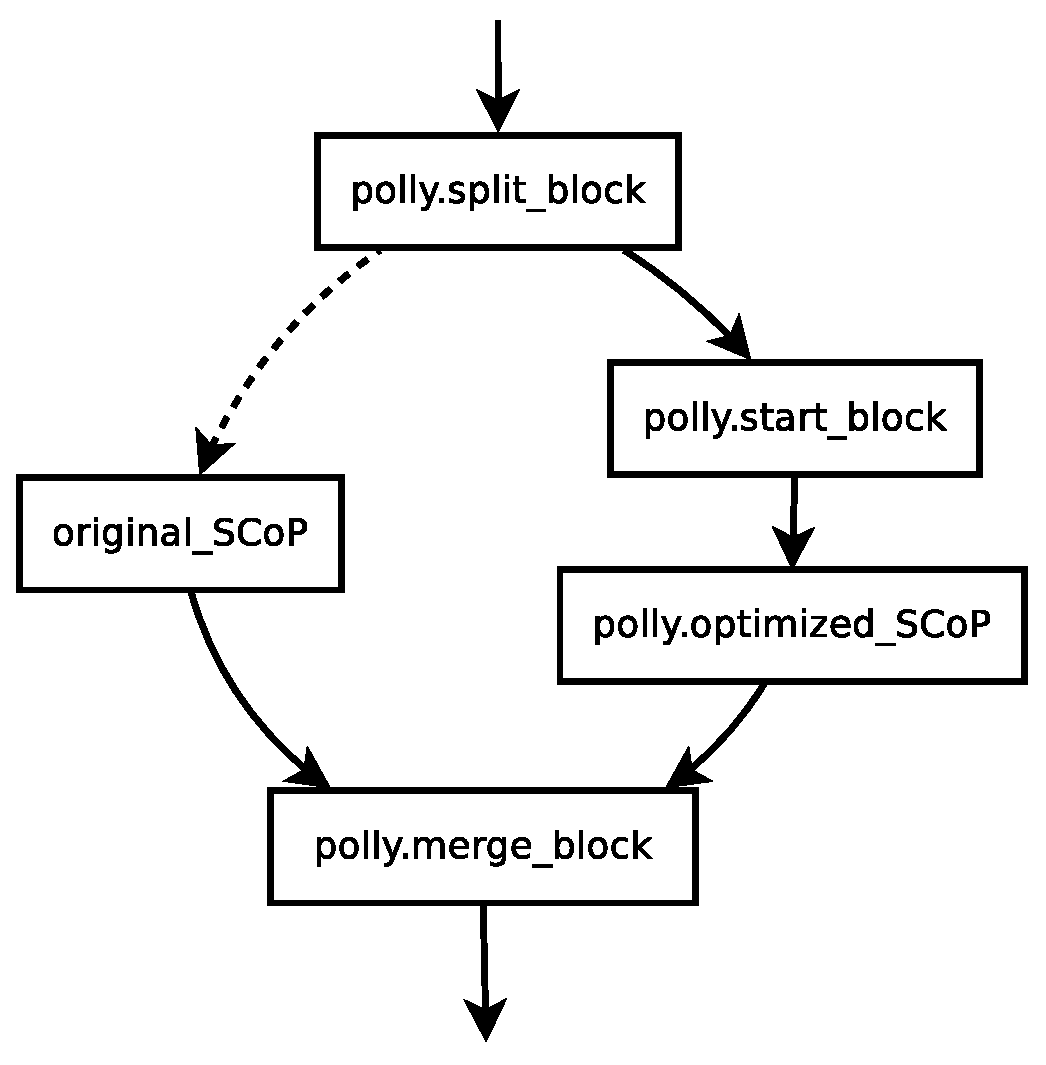
\includegraphics[width=\textwidth]{Figures/PollySCoPCFG.eps}
    \label{fig:PollySCoPCFG}
    \end{minipage}
  }
  \subfloat[SPolly optimized CFG]{
    \begin{minipage}[c][1\width]{0.45\textwidth}
    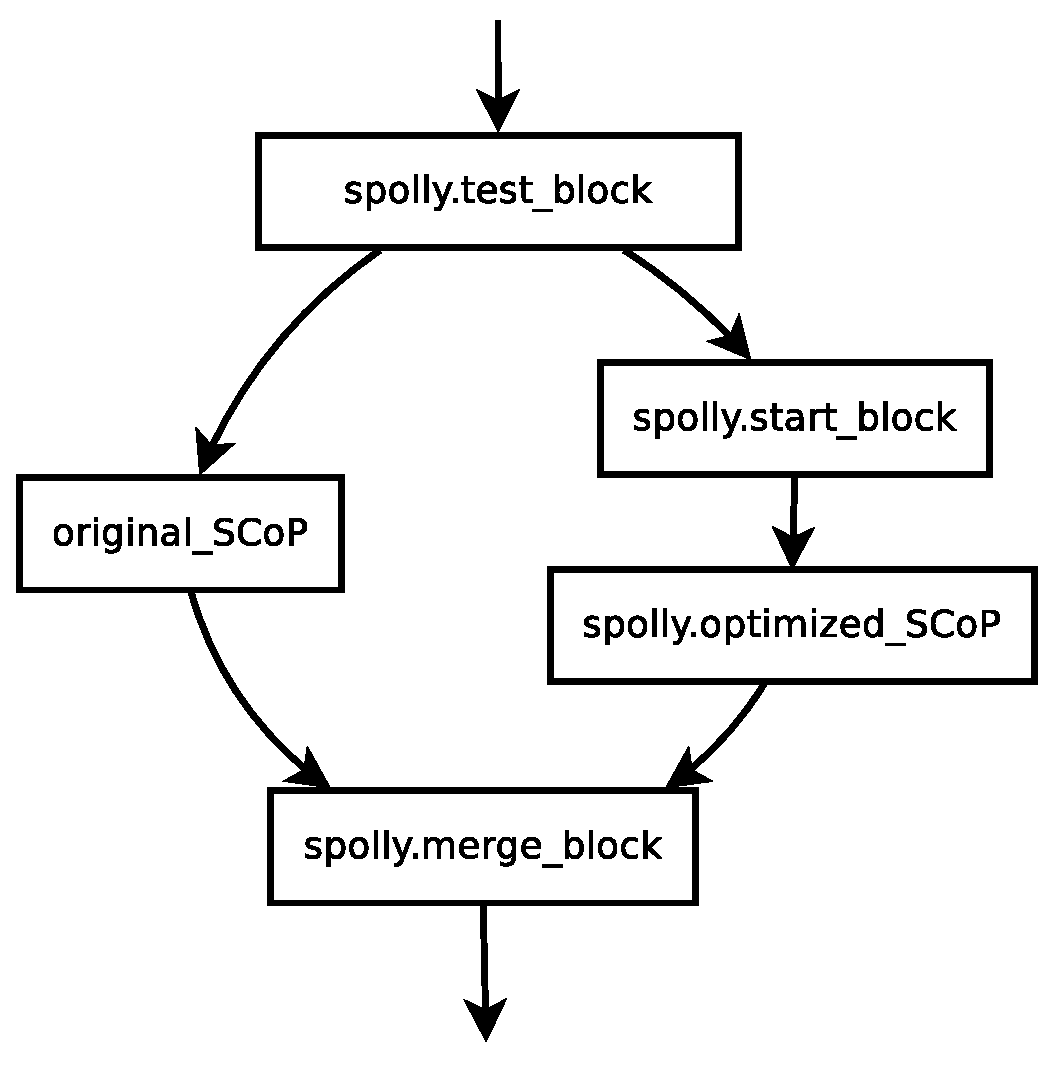
\includegraphics[width=\textwidth]{Figures/SPollySCoPCFG.eps}
    \label{fig:SPollySCoPCFG}
    \end{minipage}
  }
  \caption{CFG produced by Polly and SPolly, respectively}
  \label{fig:SCoPCFG}  
\end{figure}


\paragraph{Alias tests \\} 
~\\

Testing for aliasing pointers in general would not be feasible so another way 
was chosen. Only sSCoP invariant pointers are tested once before the sSCoP is
entered. If the test succeeds, thus no aliases are found, the optimized version
is executed. At compile time the accesses for each base pointer are collected and
marked either as possible minimal, possible maximal or not interesting access. At 
runtime all possible minimal and maximal, respectively, accesses are compared 
and the minimal and maximal access for each base pointer is computed. The alias 
test as such compares again the minimal access for a base pointer with the maximal 
accesses for the others and vice versa. At the end of this comparison chain the 
result replaces the constant guard in the split block right before the original SCoP 
and the speculative optimized one. If all base pointers are invariant in the
SCoP the test is complete, thus aliasing can be ruled out for the sSCoP at
runtime. However, non invariant pointers are not tested at all, as it would 
imply to perform all computation and testing within the loop. 
Figure \ref{fig:AliastestConcept} illustrates the concept of the alias
tests while listing \ref{lst:AliastestAccessesSrc} and figure
\ref{fig:AliastestAccesses} provide an example with the derived accesses. 
The alias test for this example would look like listing
\ref{lst:AliastestAccessesOut}.



\lstset{frame=none}
\begin{figure}[htbp]
  \centering
  \subfloat[Alias test from a birds eye view]{
  \includegraphics[width=0.9\textwidth]{Primitives/aliastest.eps}
  \label{fig:AliastestConcept}  
  }

  \vspace*{5mm}
  \subfloat[Aliasing accesses]{
    \begin{minipage}[c][3cm]{0.5\textwidth}
    \lstinputlisting{Primitives/Code/aliastestbsp.c}
    \end{minipage}
    \label{lst:AliastestAccessesSrc}  
  }
  \subfloat[Statically derived min/maximal accesses]{
    \begin{minipage}[c][3cm]{0.4\textwidth}
    \vspace*{-2mm}
    \centering
    \begin{tabular}{ c c c c }
      Acc & bp & ma & Ma \\
      \hline
      I1 & C & 0 & N$ * $N$ - 1$ \\ 
      I2 & C & 0 & N$ * $N$ - 1$\\ 
      I3 & A & 0 & N$ * $N$ - 1$\\ 
      I4 & B & 0 & N$ * $N$ - 1$\\ 
    \end{tabular}
    \end{minipage}
    \label{fig:AliastestAccesses}  
  }
  
  \subfloat[Introduced compare chain]{
    \lstinputlisting{Primitives/Code/aliastestout.c}
    \label{lst:AliastestAccessesOut}  
  }
  \caption{Alias tests concept}
  \label{fig:Aliastest}  
\end{figure}
\resetlst

\paragraph{Invariants tests \\}
~\\
Apart from alias tests, SPolly may introduce invariants tests if there are
possibly invariant variables and a function call within a sSCoP. The key idea
is to monitor possible changes in such variables during the execution of the 
profiling version. As the results may introduce new dependencies 
between loop iterations, the sSCoP could be discarded. If it does not, the sSCoP
may be optimized, depending on its new region score. As this is a 
disqualification test in the first place, the information gathered about the 
variables could be used to create specialized sSCoP versions. 
As mention earlier, the last chapter will discuss specialized versions 
in more detail. Listing \ref{lst:InvariantTestSRC} gives an example of an sSCoP 
for which invariant tests can be introduced and \ref{lst:InvariantTestOut} shows
the modified source. 


\lstset{frame=none}
\begin{figure}[htbp]
  \centering
  \subfloat[source]{
    \begin{minipage}[c][0.55\width]{0.45\textwidth}
    \lstinputlisting{Primitives/Code/InvariantTestSRC.c}
    \label{lst:InvariantTestSRC}
    \end{minipage}
  }
  \hspace*{5mm}
  \subfloat[source with invariant tests]{
    \begin{minipage}[c][0.55\width]{0.45\textwidth}
    \lstinputlisting{Primitives/Code/InvariantTest.c}
    \label{lst:InvariantTestOut}
    \end{minipage}
  }
  \caption{Invariant test introduced by SPolly}
  \label{lst:InvariantTest}  
\end{figure}
\resetlst

\paragraph{Complete Checks \\}
~\\
Alias tests may rule out aliasing in sSCoPs completely, thus some sSCoPs become
valid SCoPs after this tests are introduced. Such non speculative optimizations
are done by the compile time part of the Sambamba module and may be included in 
Polly too. An example for such an sSCoP is given in figure 
\ref{lst:AliastestAccessesSrc}. The presented code is the well known
matrix multiplication example which is a valid SCoP if the arrays do not alias.
For the sake of completeness it is to mention that this code could be
rewritten as array of pointers which would also lead to a sSCoP but without
complete checks. Chapter \ref{Chapter6} will discuss this example and the various
implementations in detail.


\subsection{Code Generation}
As part of the extension of Polly a new code generation type was added. Apart 
from sequential, vectorized and OpenMP annotated code generation SPolly is 
capable of creating a unrolled and blocked loop, which can be easily 
translated into an ParCFG, thus parallelized by a Sambama module. Listing 
\ref{lst:ForkJoinCodeGenerationOUT} presents this transformation. The special 
case where lower and upper bound as well as the 
stride are statically known constants, the second loop, which computes 
remaining iterations, is completely unrolled.
This kind of loop unrolling and blocking may find its 
way into Polly in the near future. 

\subsubsection*{Parallelization}

In order to secure the speculative executions with Sambambas STM
(see \ref{SambambaSTM}) the Sambama parallelizer needs to be used.
As this parallelizer does not yet support loop parallelization per se, some 
transformation needed to be done first. The new code generation type was created
to do the difficult one without recomputing information provided during by the
polytope model (during the code generation) anyway. As these transformation
yields code as in listing \ref{lst:ForkJoinCodeGenerationOUT} the creation of
a ParCFG (see \ref{SambambaParCFG}) remains. Figures \ref{fig:ForkJoinCFG} and
\ref{fig:ForkJoinParCFG} visualize these changes.


\lstset{frame=none}
\begin{figure}[htbp]
  \centering
  \subfloat[Initial loop nest]{
    \begin{minipage}[c][1\width]{0.45\textwidth}
    \lstinputlisting{Primitives/Code/ForkJoinCodeGenerationSRC.c}
    \label{lst:ForkJoinCodeGenerationSRC}
    \end{minipage}
  }
  \subfloat[Listing \ref{lst:ForkJoinCodeGenerationSRC} after N-fork creation]{
    \begin{minipage}[c][1\width]{0.45\textwidth}
    \lstinputlisting{Primitives/Code/ForkJoinCodeGenerationOUT.c}
    \label{lst:ForkJoinCodeGenerationOUT}
    \end{minipage}
  }

  \subfloat[SPolly forked CFG]{
    \begin{minipage}[c][8cm]{0.40\textwidth}
    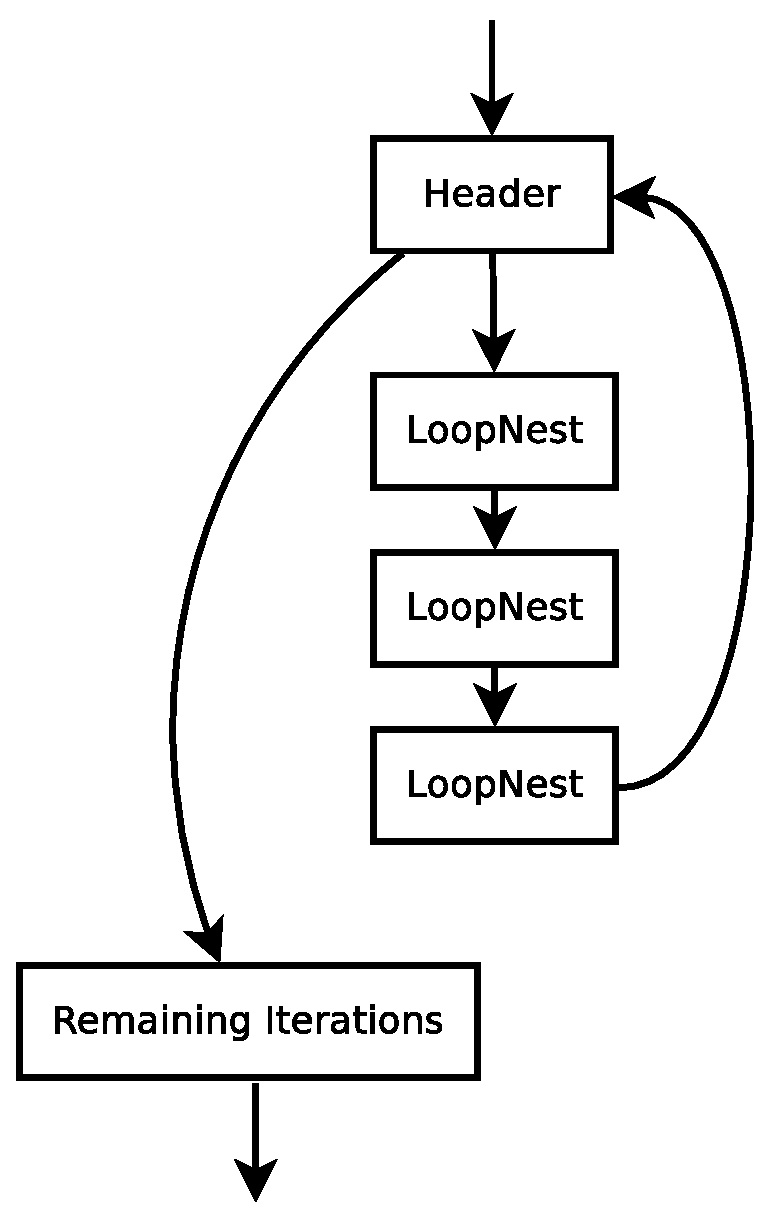
\includegraphics[width=0.7\textwidth]{Figures/ForkJoinCFG.eps}
    \label{fig:ForkJoinCFG} 
    \end{minipage}
  }
  \subfloat[SPolly ParCFG]{
    \begin{minipage}[c][8cm]{0.50\textwidth}
    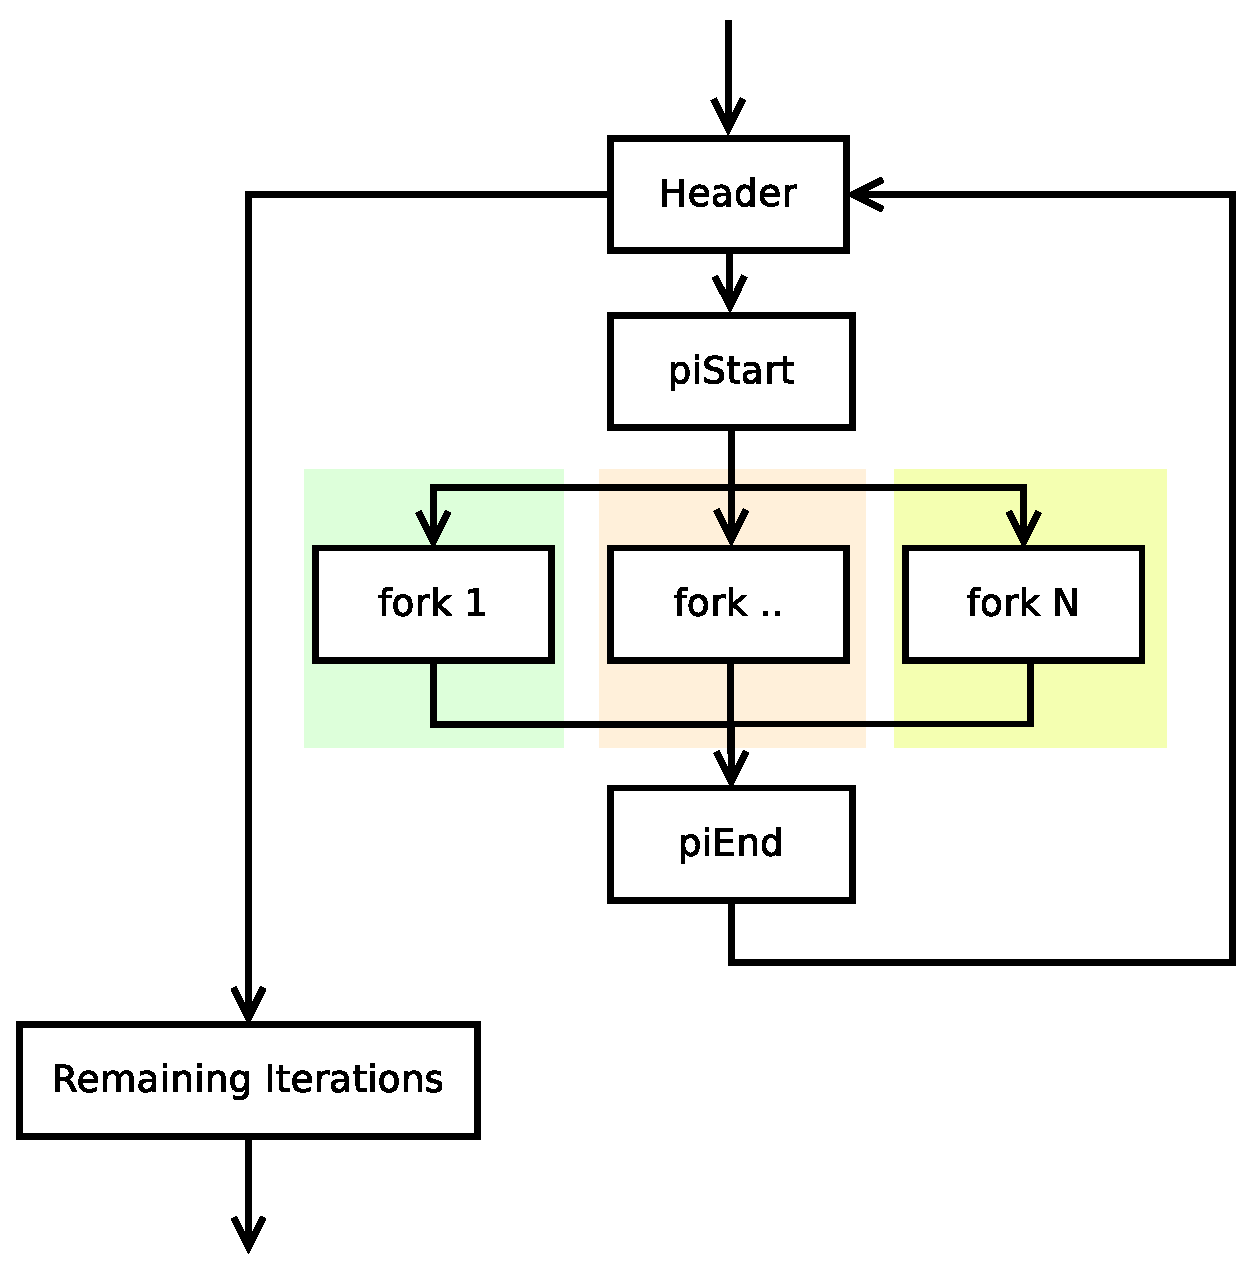
\includegraphics[width=\textwidth]{Figures/ForkJoinParCFG.eps}
    \label{fig:ForkJoinParCFG}
    \end{minipage}
  }
  \caption{Forked CFG produced by SPolly and resulting ParCFG}
  \label{fig:CreateParCFG}  
\end{figure}
\resetlst

\section{Sambama Compile Time Module}
The compile time part of the Sambamba module locates all sSCoPs
within the given input module and transfers each one afterwards in a separated 
function. These extracted sSCoPs are stored within the created Sambamba 
bitcode or respectively executable file. Extracting every single sSCoP 
decreases the performance but allows to easily change and combine different 
optimized sSCoPs, even if they originated from the same function.   
At the moment there is one exception implemented which will be applied on sSCoPs
with complete checks, thus valid SCoPs after the tests are passed. All of those
are optimized in place without consulting the region scores or any other heuristic.
The functionality of the compile time part is minimal but it helps to focus 
on profiling and execution during runtime, without analysis overhead. 
Further work could heavily improve this part, beginning by compile time 
preparation of the sSCoPs, but imaginable is more than just a precomputed
profiling or optimized version of a sSCoP.
As there are a lot of parameters which could have significant impact 
on the performance, several optimized versions of an sSCoP could be created
and stored, in order to choose the best depending on the system and the actual
run, thus depending on runtime information.
While table \ref{tab:PollyOptions} gives a brief
overview of available options for Polly, it is not clear which ones will
fit best for a particular environment and sSCoP. 
As the method versioning system of Sambamba evolves, the compile time part 
should, in order to reduce the workload at runtime and increase the ability to
adapt. 

\section{Sambama Runtime Module}

In addition to the compile time parts, which only rely on static analyses,
the runtime part uses different kinds of runtime information to decide. 
To take advantage of this extra knowledge, most of the decisions, thus most of
the program logic, is implemented in the runtime module. 


Table \ref{}[TODO] gives an overview of the functionalities.


\begin{table}[htbp]
  \caption{Functionality of the SPolly Sambamba module}
  \begin{tabular}{| l |}
    \hline
    
    \hline
    \hline

    \hline
  \end{tabular}
\end{table}



\subsection{Profiling}


\section{Profiling For Sambamba}

Sambamba, as heavily developed research project, was not capable of any kind
of profiling when I started my work. By now, there are two profilers available.
The first one, implemented by the authors of Sambamba, 
is used for exact time measuring, while I created the second one to profiles
executions and data.
[TODO if first is used later on, write it here] Both were
developed during the same time to fulfill different needs and could be
[TODO will be ?]  merged anytime soon. 
As most of SPollys parts are unrelated, to both of them, 
the profiling versions, as their name indicates, would become useless without.
This will definitely increase the number of unnecessary created (parallel) 
functions, but it would not render SPolly redundant.
There a sSCoPs which a guarded by sound checks, thus they can be used with the
overhead of only the check. As the use of other sSCoPs could increase the 
performance too, a heuristic could look for promising candidates, even without
any runtime information. This heuristic could be part of future work since even
with a profiler by hand, there are cases where the gathered information
(see [TODO]) are not helpful at all.



\section{Region Scores}
Initial efforts to create these scores did not use any kind of 
memory, thus the whole region was analysed every time new information was available.
To avoid this unnecessary computations the current score is a
symbolic value which may contain variables for values not known statically, e.g.,
branch probabilities or loop bounds.
Evaluation of these symbolic values will take all profiling 
information into account and yield a comparable integer value. 
Only during the initial score creation the region will be traversed to find
parameters and branches for later annotation. 

All instructions will be scored and the violating ones
will be checked for their speculative potential.
As memory instructions are 
guarded by the STM for the case the speculation failed, calls may not be
reversible, thus without any speculative potential at all. Such function calls
are not checked earlier since the region speculation needs the information about
possible other branches within this region. 
Listing \ref{lst:sSCoPprintf} 
provides such an example but these cases will be revisited in the next 
two chapters too. Table \ref{tab:Scores} lists the scores for the examples in 
figure \ref{fig:ScoredSCoPs}.

